\documentclass[border=5pt,tikz]{standalone}
\usepackage{amsmath} % for \dfrac
\usepackage{physics}
\usepackage{tikz}
% \pgfplotsset{compat=1.18}
%\usepackage[outline]{contour} % glow around text
\usetikzlibrary{arrows,arrows.meta}
% \usetikzlibrary{decorations.markings}
% \usetikzlibrary{hobby}
% \usepgfplotslibrary{fillbetween}
\usetikzlibrary{decorations.pathmorphing}
\usepackage[detect-all]{siunitx}

\begin{document}
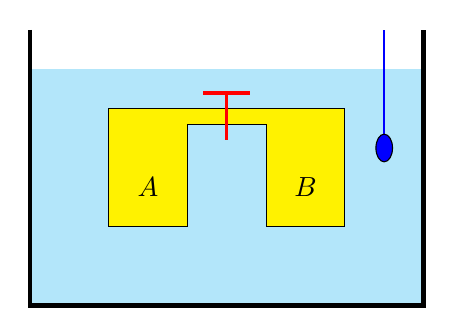
\begin{tikzpicture}
  \fill[cyan!30]
        {
        }
        (0, 0) -- (5, 0) -- (5, 3) -- (0, 3) -- cycle;
    \draw[ultra thick] (0, 3.5) -- (0, 0) -- (5, 0) -- (5, 3.5);
    \draw[draw=black, fill=yellow] (1, 2.5) -- (1, 1) -- (2, 1) -- (2, 2.3) -- (3, 2.3) -- (3, 1) -- (4, 1) -- (4, 2.5) -- cycle ;
    
    \draw[very thick, red] (2.2, 2.7) -- (2.8, 2.7);
    \draw[very thick, red] (2.5, 2.7) -- (2.5, 2.1);

    \draw[thick, blue] (4.5, 2) -- (4.5, 3.5);
    \draw[black, fill = blue] (4.5, 2) ellipse (3 pt and 5 pt);
    
    \node[] at (1.5, 1.5) {$A$};
    \node[] at (3.5, 1.5) {$B$};
\end{tikzpicture}
\end{document}